\documentclass{article}
\usepackage[margin=1in]{geometry}
\usepackage{amsmath,amssymb}
\usepackage{parskip}
\usepackage{graphicx}
\usepackage{caption}
\usepackage{booktabs}
\DeclareMathOperator*{\argmin}{arg\,min}
\DeclareMathOperator*{\argmax}{arg\,max}

\title{CSE P 546 A - Homework 1}
\author{Thangakumar Dhanasekaran (2550520)}
\date{Apr-19-2026}

\begin{document}

\maketitle

\section*{A1}

\subsection*{(a) Bias, Variance, and the Bias-Variance Tradeoff}

\textbf{Bias} is the error introduced by a model's simplifying assumptions. It reflects how far off the model's predictions are from the true values on average.\\ \textbf{Variance} is the model's sensitivity to fluctuations in the training data --- a high-variance model changes dramatically with different training sets.\\ The \textbf{bias-variance tradeoff} is the tension between these two: reducing bias (making the model more flexible) tends to increase variance, and vice versa, so the goal is to find a balance that minimizes total error.

\subsection*{(b) Effect of Model Complexity on Bias and Variance}

As model complexity \textbf{increases}, bias decreases (the model can fit more nuanced patterns) but variance increases (it overfits the training data). As complexity \textbf{decreases}, bias increases (the model is too rigid) while variance decreases (it becomes more stable across datasets).

\subsection*{(c) True or False: A learning algorithm will always generalize better if we use fewer features}

\textbf{False.} Using fewer features does not guarantee better generalization. If the removed features are genuinely informative, discarding them increases bias and hurts performance. Feature selection must be done carefully --- the right features matter, not simply fewer ones.

\subsection*{(d) True or False: Hyperparameters should be tuned on the test set}

\textbf{False.} Hyperparameters should \textbf{not} be tuned on the test set, as this causes data leakage --- the test set would no longer be an unbiased estimate of generalization error. The standard procedure is \textbf{$k$-fold cross-validation} on the training set: split the training data into $k$ folds, train on $k{-}1$ folds and validate on the remaining fold, repeat $k$ times, and select the hyperparameters with the best average validation performance. The test set is touched only once, at the very end, to report final performance.

\subsection*{(e) True or False: The training error of a function on the training set provides an overestimate of the true error of that function}

\textbf{False.} Training error typically \textbf{underestimates} true (generalization) error, not overestimates it. Because the model was fit to the training data, it performs artificially well on it --- especially for complex models that overfit --- leading to optimistically low training error compared to error on unseen data.


\section*{A2 --- Maximum Likelihood Estimation (MLE)}

\subsection*{(a) Deriving the MLE for $\lambda$}

\paragraph{Setup.}
We observe $n$ i.i.d.\ goal counts $x_1, \ldots, x_n$, each modelled as Poisson($\lambda$):
\[
  \Pr(X = x \mid \lambda) = \frac{e^{-\lambda}\,\lambda^{x}}{x!}, \qquad x = 0,1,2,\ldots, \quad \lambda > 0.
\]

\paragraph{Step 1: Write the likelihood.}
Because the observations are i.i.d., the joint likelihood is the product of the individual probabilities:
\[
  L(\lambda)
  = \prod_{i=1}^{n} \frac{e^{-\lambda}\,\lambda^{x_i}}{x_i!}
  = e^{-n\lambda}
    \cdot \lambda^{\,\sum_{i=1}^{n} x_i}
    \cdot \underbrace{\prod_{i=1}^{n} \frac{1}{x_i!}}_{\text{constant w.r.t.\ }\lambda}.
\]

\paragraph{Step 2: Take the log-likelihood.}
Since $\log$ is strictly monotone increasing, $\arg\max L(\lambda) = \arg\max \ell(\lambda)$
where $\ell(\lambda) = \log L(\lambda)$:
\begin{align*}
  \ell(\lambda)
  &= \log e^{-n\lambda}
     + \log \lambda^{\,\sum_{i=1}^n x_i}
     + \log \prod_{i=1}^n \frac{1}{x_i!} \\
  &= -n\lambda
     + \left(\sum_{i=1}^n x_i\right)\log\lambda
     - \sum_{i=1}^n \log(x_i!).
\end{align*}
The last term is constant in $\lambda$ and plays no role in the optimisation.

\paragraph{Step 3: Differentiate and set equal to zero.}
\[
  \frac{d\ell}{d\lambda}
  = -n + \frac{\displaystyle\sum_{i=1}^n x_i}{\lambda} = 0.
\]

\paragraph{Step 4: Solve for $\hat{\lambda}$.}
\[
  \frac{\displaystyle\sum_{i=1}^n x_i}{\lambda} = n
  \;\implies\;
  \boxed{\hat{\lambda}_{\text{MLE}} = \frac{1}{n}\sum_{i=1}^n x_i = \bar{x}.}
\]
The MLE is the \textbf{sample mean} --- intuitive because $\mathbb{E}[X] = \lambda$ for a Poisson
distribution. The MLE is finite provided $\sum x_i > 0$ (satisfied here: $\sum x_i = 13$).

\paragraph{Step 5: Confirm global maximum.}
\[
  \frac{d^2\ell}{d\lambda^2}
  = -\frac{\displaystyle\sum_{i=1}^n x_i}{\lambda^2} < 0
  \quad (\text{since } \textstyle\sum x_i > 0,\; \lambda^2 > 0).
\]
The log-likelihood is strictly concave at the critical point, confirming $\hat{\lambda}_{\text{MLE}}$
is the unique global maximum.

\subsection*{(b) Numerical estimate of $\lambda$ after five games}

The observed scores are $[2, 4, 6, 0, 1]$, so:
\[
\hat{\lambda} = \frac{2 + 4 + 6 + 0 + 1}{5} = \frac{13}{5} = 2.6
\]

The probability that the Reign score 6 goals in their next game:
\[
\text{Poi}(6 \mid 2.6) = e^{-2.6} \cdot \frac{2.6^6}{6!} \approx \mathbf{0.0319}
\]

\subsection*{(c) Updated estimate after six games (8 goals in game 6)}

With scores $[2, 4, 6, 0, 1, 8]$:
\[
\hat{\lambda} = \frac{2 + 4 + 6 + 0 + 1 + 8}{6} = \frac{21}{6} = 3.5
\]

The probability that the Reign score 6 goals in their 7th game:
\[
\text{Poi}(6 \mid 3.5) = e^{-3.5} \cdot \frac{3.5^6}{6!} \approx \mathbf{0.0771}
\]

\section*{A3: Effect of Regularization}

\begin{figure}[h]
    \centering
    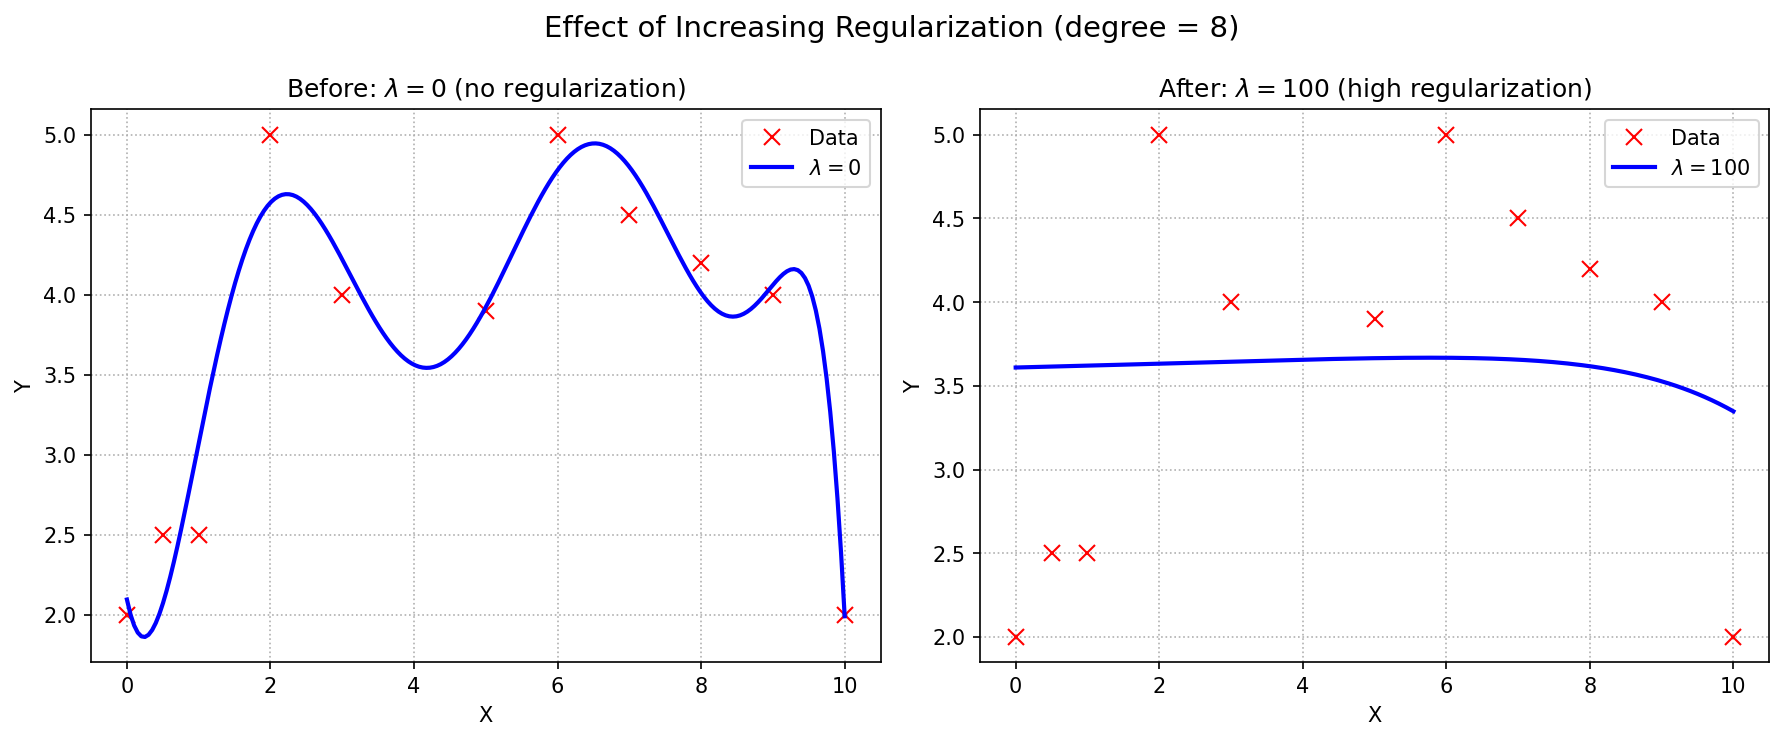
\includegraphics[width=\textwidth]{reg_effect.png}
    \caption{Degree-8 polynomial fit with $\lambda=0$ (left) versus $\lambda=100$ (right) on the polyreg dataset.}
\end{figure}

Increasing the regularization parameter $\lambda$ shrinks the model weights toward zero, causing the high-degree polynomial to produce a much smoother, flatter curve that trades variance for bias---eliminating the wild oscillations seen when $\lambda=0$ but at the cost of underfitting the underlying trend.

\section*{A4: Bias-Variance Tradeoff via Learning Curves}

\begin{figure}[h]
    \centering
    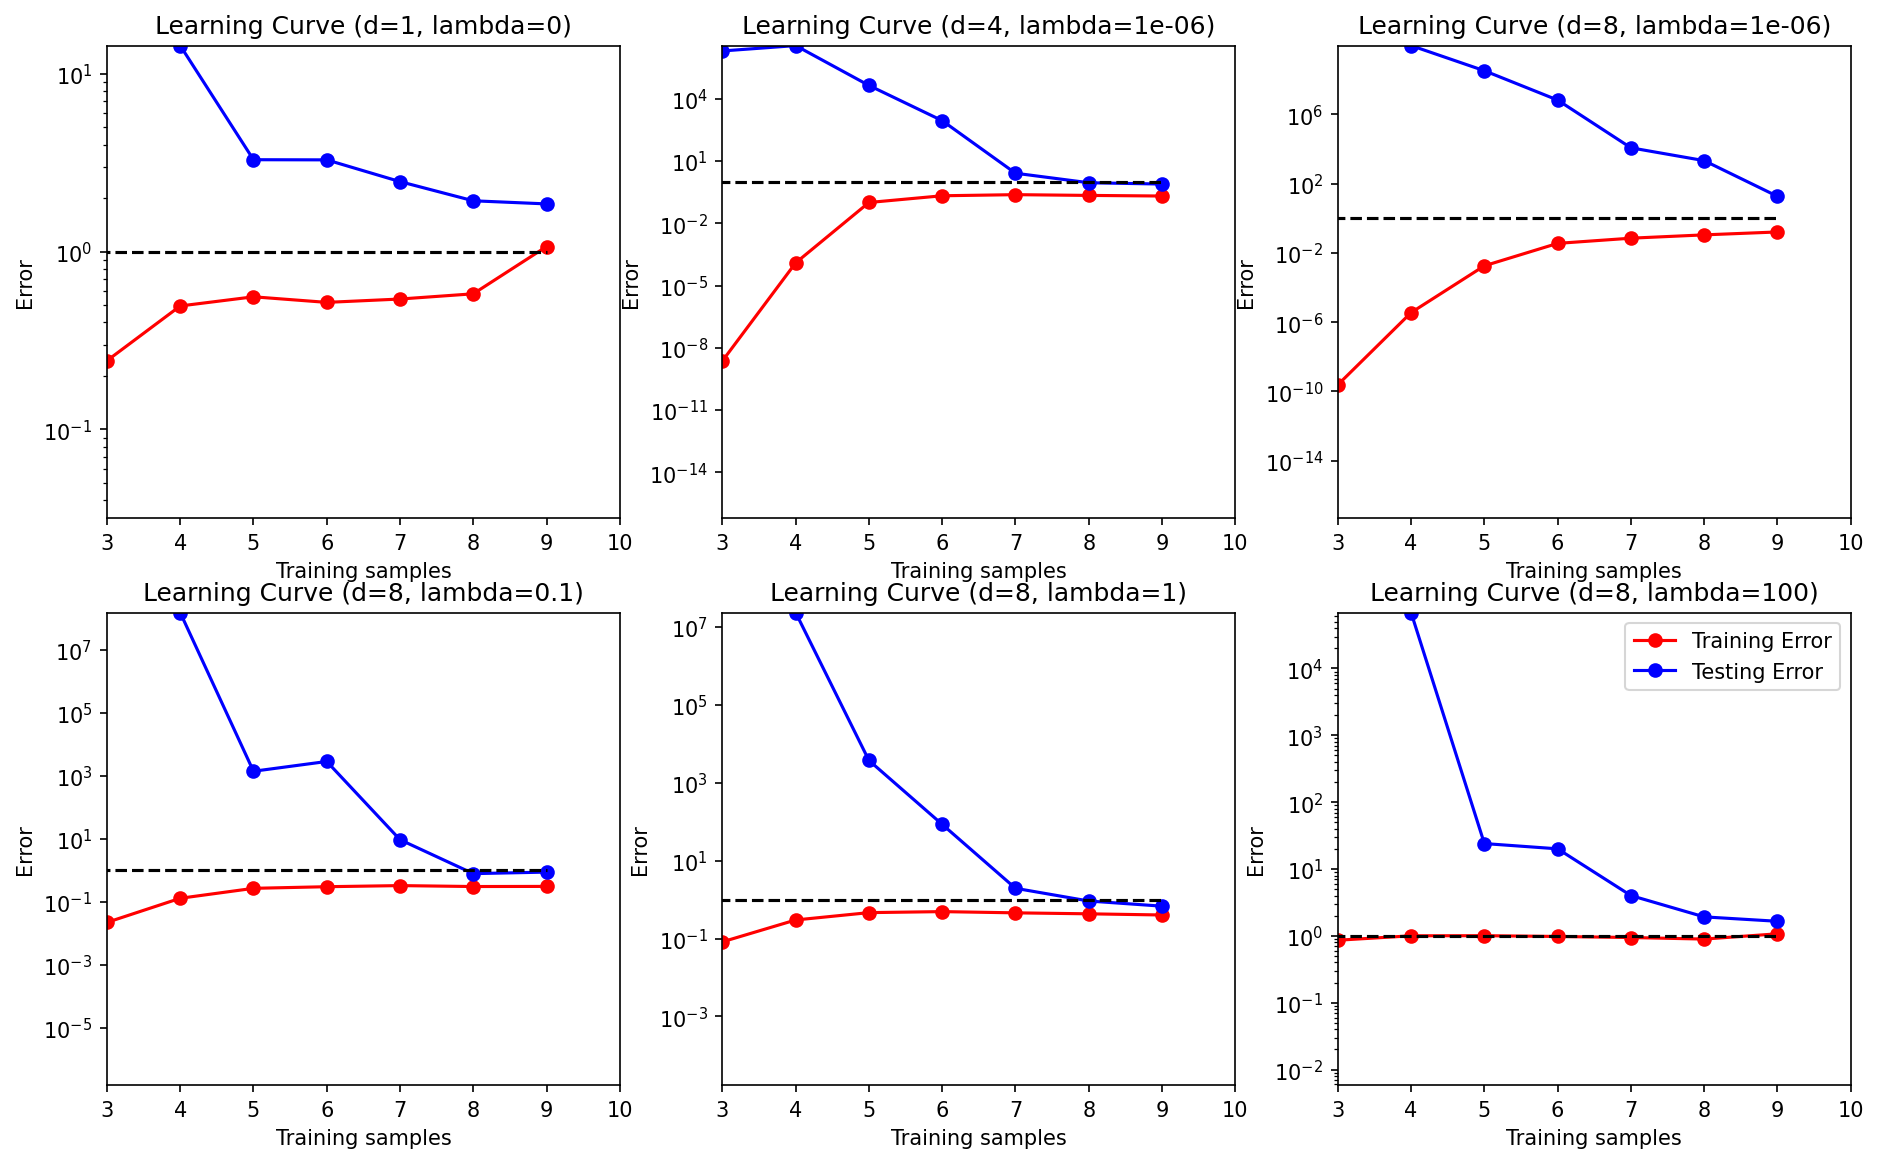
\includegraphics[width=\textwidth]{learning_curves.png}
    \caption{Learning curves (training error in red, test error in blue) for six combinations of polynomial degree $d$ and regularization $\lambda$.}
\end{figure}

As $\lambda$ increases from $10^{-6}$ to $100$ (degree $d=8$ panels), the gap between training and test error narrows because regularization reduces overfitting, but both errors converge to a higher floor, indicating that too much regularization introduces bias and prevents the model from capturing the true signal.


\clearpage
\section*{A5 --- Ridge Regression on MNIST}

\subsection*{(a) Derivation of $\hat{W} = (X^\top X + \lambda I)^{-1} X^\top Y$ \hfill [10 pts]}

We wish to find
\[
  \hat{W} = \argmin_{W \in \mathbb{R}^{d \times k}}
  \sum_{i=1}^{n} \bigl\|W^\top x_i - y_i\bigr\|_2^2
  + \lambda \|W\|_F^2.
\]

\paragraph{Step 1: Decompose the objective column-wise.}
Write $w_j = W e_j$ for the $j$-th column of $W$ (so $W = [w_1 \; \cdots \; w_k]$).
Using the identity $\|W\|_F^2 = \sum_{j=1}^k \|w_j\|_2^2$, the objective separates into
$k$ independent sub-problems:
\begin{align*}
  \sum_{i=1}^n \|W^\top x_i - y_i\|_2^2 + \lambda\|W\|_F^2
  &= \sum_{j=1}^{k}
     \left[
       \sum_{i=1}^n \bigl(e_j^\top W^\top x_i - e_j^\top y_i\bigr)^2
       + \lambda\|w_j\|_2^2
     \right] \\
  &= \sum_{j=1}^{k}
     \Bigl[
       \|Xw_j - Ye_j\|_2^2 + \lambda\|w_j\|_2^2
     \Bigr],
\end{align*}
where $X = [x_1 \;\cdots\; x_n]^\top \in \mathbb{R}^{n \times d}$ and
$Y = [y_1 \;\cdots\; y_n]^\top \in \mathbb{R}^{n \times k}$.

\paragraph{Step 2: Minimize each sub-problem.}
Because the $k$ sub-problems share no variables, we may minimize each independently.
For a fixed $j$, expand the cost:
\[
  f_j(w_j)
  = \|Xw_j - Ye_j\|_2^2 + \lambda\|w_j\|_2^2
  = w_j^\top (X^\top X + \lambda I)\, w_j
    - 2\,(Ye_j)^\top X w_j
    + \|Ye_j\|_2^2.
\]
Since $X^\top X \succeq 0$ and $\lambda > 0$, the matrix $(X^\top X + \lambda I)$ is
strictly positive definite, so $f_j$ is strictly convex and has a unique minimum.
Setting the gradient to zero:
\[
  \nabla_{w_j} f_j(w_j)
  = 2(X^\top X + \lambda I)\,w_j - 2 X^\top Y e_j = 0
  \;\implies\;
  (X^\top X + \lambda I)\,\hat{w}_j = X^\top Y e_j.
\]
Because $(X^\top X + \lambda I)$ is invertible (positive definite), the unique solution is
\[
  \hat{w}_j = (X^\top X + \lambda I)^{-1} X^\top Y e_j.
\]

\paragraph{Step 3: Reassemble the full weight matrix.}
Stacking the $k$ column solutions side by side:
\begin{align*}
  \hat{W}
  &= \bigl[\hat{w}_1 \;\cdots\; \hat{w}_k\bigr] \\
  &= \bigl[(X^\top X + \lambda I)^{-1} X^\top Y e_1
     \;\cdots\;
     (X^\top X + \lambda I)^{-1} X^\top Y e_k\bigr] \\
  &= (X^\top X + \lambda I)^{-1} X^\top Y\,
     \underbrace{[e_1 \;\cdots\; e_k]}_{= I_k} \\[4pt]
  &= \boxed{(X^\top X + \lambda I)^{-1} X^\top Y.}
\end{align*}

\subsection*{(b) Training and Testing Errors \hfill [10 pts]}

Using the closed-form $\hat{W}$ derived above, we train a multi-class ridge regression
classifier on the MNIST dataset ($n = 60{,}000$ training images,
$n_{\text{test}} = 10{,}000$ test images, $d = 784$ pixel features, $k = 10$ classes)
with regularization parameter $\lambda = 10^{-4}$.
Labels are one-hot encoded before training.
Predicted class for observation $x$ is $\hat{z} = \argmax_j\, e_j^\top \hat{W}^\top x$.

\begin{center}
\begin{tabular}{lc}
\toprule
\textbf{Split} & \textbf{Classification Error} \\
\midrule
Train ($n = 60{,}000$) & $14.805\%$ \\
Test  ($n = 10{,}000$) & $14.660\%$ \\
\bottomrule
\end{tabular}
\end{center}

Both errors are approximately $14.7\%$, consistent with the expected ${\sim}15\%$
reported in the problem statement.
The near-identical train and test errors indicate that the model does not overfit ---
the regularization $\lambda = 10^{-4}$ is effective.
The residual error reflects the intrinsic limitation of a linear decision boundary in
raw pixel space: the model cannot represent the nonlinear structure of handwritten
digits, so a substantial irreducible error remains for all choices of $\lambda$.

\end{document}
